% L22eqv.tex
%
% Predrag created file              jul  9 2006
% $Author$ $Date$


\section{Small $L=22$ system {\rpo s}}
\label{s:L22}


\KS\ system with $L = 22$ periodic on the full space is small but
empirically large enough to exhibit persistent chaos.  $L=22$ is a
sensible choice because in units of mean wavelength the size of this
small system is about 2.5 wavelengths ($\tildeL/\sqrt{2}= 2.4758$),
so the dynamics is a competition between wavenumbers 2 and 3.
Because of the strong $k^4$ contraction in \KS\ we expect a small
number of eigenvalues to be significant for the dynamics, while the
rest are in the numerical noise. See figure~6 in
\refref{Christiansen:97}.

%% Davidchack and Crofts
% We investigate this system in 16 to 64 complex Fourier modes (32 to
%128-dimensional system of real ODEs) truncation, and recheck the results
%by redoing the calculation with the double number of Fourier modes. %
%observe how many digits change. The \eqv\ points are accurate to at least
%to $10^{-11}$. Since Lapack is also double precision accurate, the
%accuracy of the first few eigenvalues is similar, and certainly in excess
%of 6 significant digits. % All digits stated in tables are significant.
%The accuracy that can be reached is of order of
%$|a(\period{p},d_p) - a_0|
% \approx \epsilon \exp(\Lyap_p \period{p})$,
% where $\epsilon \approx 10^{-17}$ for double precision, $\Lyap_p$ is
%the largest Lyapunov exponent, and $\period{p}$ the period.  With a good
%starting guess, Newton's method typically reaches that accuracy after 2-3
%iterates.

\subsection{\Eqva}

In addition to the trivial \eqv\ $u=0$ (denoted \EQV{0} from now
on), we find for $L = 22$ three \eqva\ with dominant wavenumber $k$
(denoted \EQV{k}) for $k = 1, 2, 3$.  All {\eqva}, shown in
Fig.~\ref{f:KS22Equil}, are symmetric with respect to the reflection
symmetry. The \eqva\ \EQV{2} and \EQV{3} have additional symmetry with respect
to translation by $L/2$ and $L/3$, respectively.

\begin{figure}[t]
\begin{center}
(a)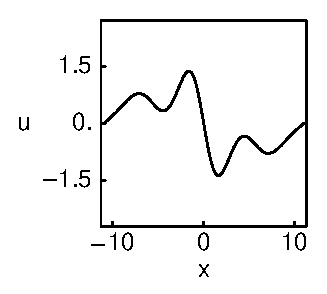
\includegraphics[width=0.25\textwidth]{figs/1wKS22equil.eps}
(b)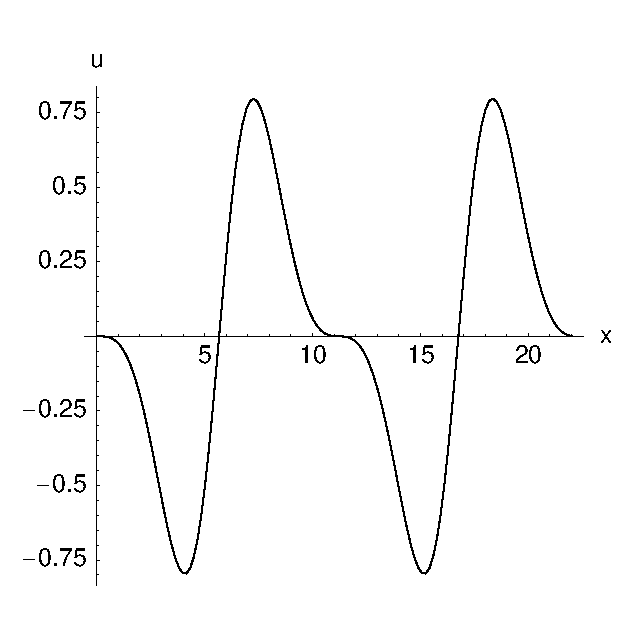
\includegraphics[width=0.25\textwidth]{figs/2wKS22equil.eps}
(c)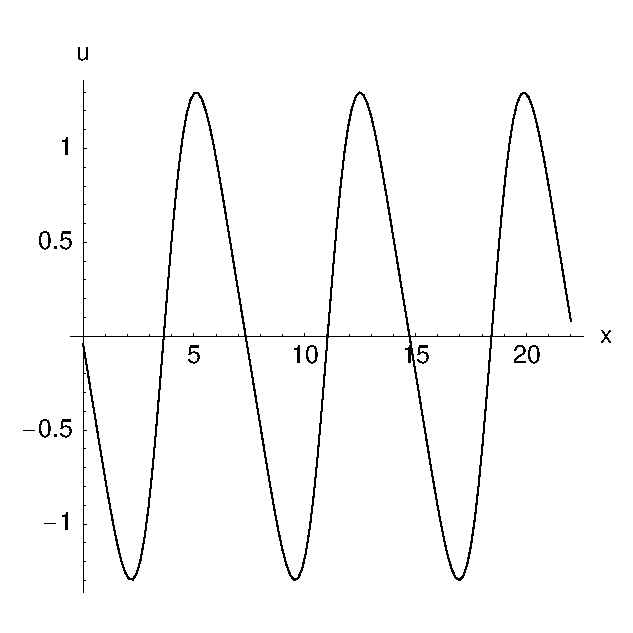
\includegraphics[width=0.25\textwidth]{figs/3wKS22equil.eps}
\end{center}
\caption{
(a) \EQV{1}, (b) \EQV{2}, and (c)
\EQV{3} \eqva\ of \KS\ equation.
% with $L=22$.
}
\label{f:KS22Equil}
\end{figure}

The stability of the {\eqva} is characterized by the eigenvalues
$\lambda_j$ of the Jacobian matrix.  First ten eigenvalues for each
\eqv\ are listed in \reftab{tab:EkEigs} in the order of
decreasing real parts. Recall that an \eqv\ with $\mathrm{Re}
\lambda_j > 0$ is unstable in the direction of the corresponding
eigenvector $\jEigvec{j}$.

\begin{table}[t]\label{tab:EkEigs}
\begin{center} \footnotesize
\caption{ Eigenvalues of the \eqva\ for $L=22$.}
\begin{tabular}{cccc} \hline
  \EQV{0}  &    \EQV{1}        &    \EQV{2}        &  \EQV{3}   \\\hline
  $0.2198$ &  $0.1308+i0.3341$ &  $0.1390+i0.2384$ &  $0.0933$\\
  $0.2198$ &  $0.1308-i0.3341$ &  $0.1390-i0.2384$ &  $0.0933$\\
  $0.1952$ &  $0.0824+i0.3402$ &  $0$              &  $0$\\
  $0.1952$ &  $0.0824-i0.3402$ & $-0.0840+i0.1602$ & $-0.4128$\\
  $0.0749$ &  $0$              & $-0.0840-i0.1602$ & $-0.6108+i0.3759$\\
  $0.0749$ & $-0.2287+i0.1963$ & $-0.1194$         & $-0.6108-i0.3759$\\
 $-0.3981$ & $-0.2287-i0.1963$ & $-0.2711+i0.3563$ & $-0.6108+i0.3759$\\
 $-0.3981$ & $-0.2455$         & $-0.2711-i0.3563$ & $-0.6108-i0.3759$\\
 $-2.1191$ & $-2.0554$         & $-2.0130$         & $-1.6641$\\
 $-2.1191$ & $-2.0619$         & $-2.0378$         & $-1.6641$\\\hline
\end{tabular}
\end{center}
\end{table}

The eigenvalues of \EQV{0} are determined by the linear part of the KS
equation: $\lambda_k=q_k^2-q_k^4$, where $q_k = 2\pi k/L$.  For
$L=22$, there are three pairs of unstable eigenvalues: corresponding
to three unstable modes $k=2,3$, and 1, respectively.  For each
mode, the corresponding eigenvectors lie in the plane spanned by
$\mathrm{Re} a_k$ and $\mathrm{Im} a_k$. \refTab{tab:E1sym} to \reftab{tab:E3sym}
list the symmetries corresponding to the stability eigenvectors of
\eqva\ \EQV{1} to \EQV{3}.
With $S$, $A$ we denote an eigenvector belonging to the symmetric
or antisymmetric subspace respectively. The last column lists
the symmetry expected to be present in the corresponding
stable/ustable manifold.

\PCedit{I suggest moving \reftab{tab:EkEigs} and related into Appendix,
replacing them with figures like Gibson's
\reffig{f:KS22EkEigs}.
    }

\begin{figure}[t]
\begin{center}
(a)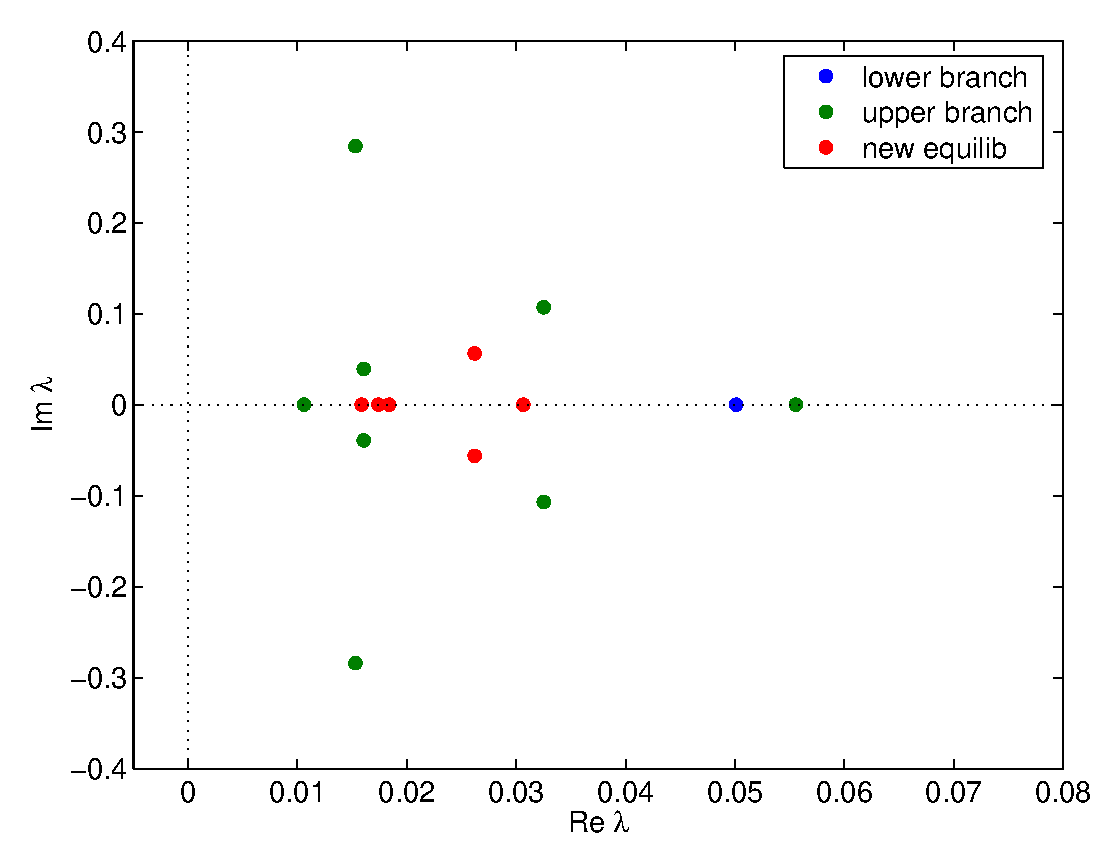
\includegraphics[width=0.45\textwidth]{figs/lambdaUnstab}
(b)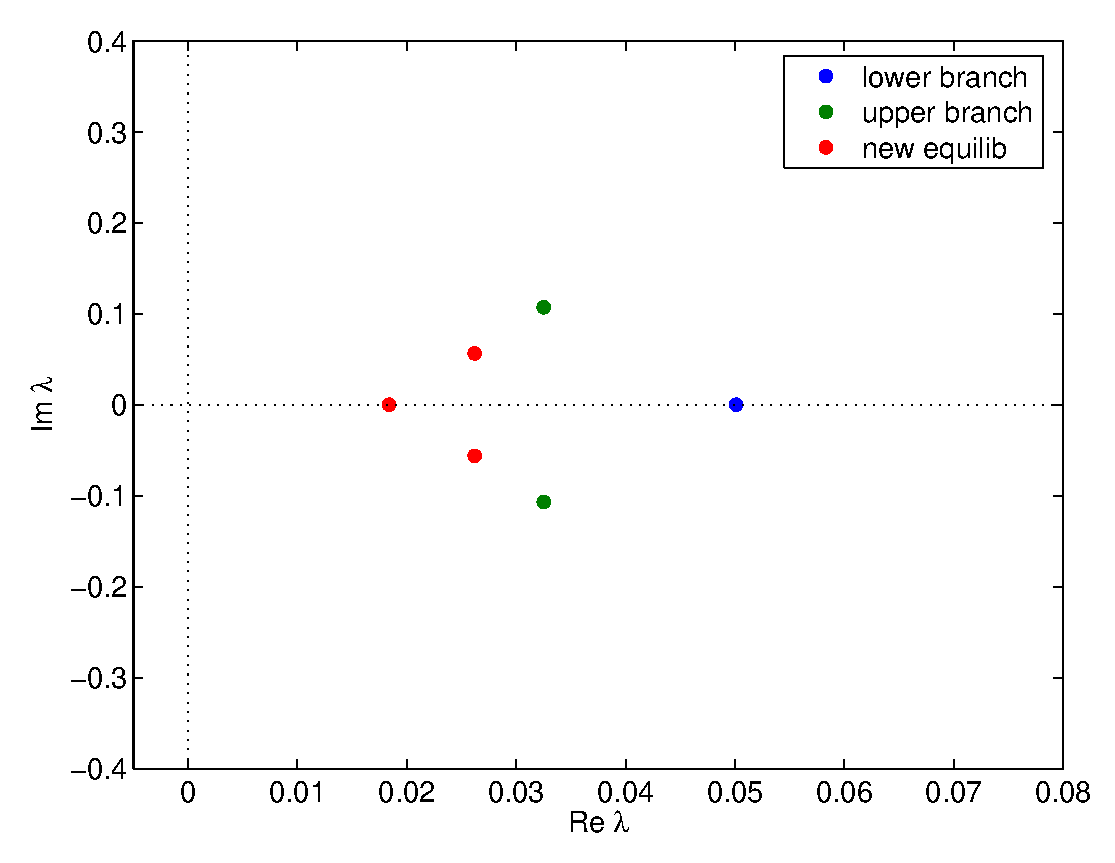
\includegraphics[width=0.45\textwidth]{figs/lambdaUnstabSymm.eps}
\end{center}
\caption{
(a) Stability eigenvalues of all \eqva\ and \reqva.
(b) Eigenvalues of \eqva\ and \reqva\ within
the symmetric subspace $R_1$.
}
\label{f:KS22EkEigs}
\end{figure}

\begin{table}[t]\label{tab:E1sym}
\caption{
Leading eigenvalues and symmetries of the eigenspaces of \KS\ equation {\eqva} with $L = 22$. We have used as our reference states the ones that lie on the antisymmetric subspace and also listed the symmetries of the $L/4$ translated ones.
        }
\begin{center} \footnotesize
\begin{tabular}{ccccc} \hline
\EQV{1}& $\mathrm{Re} \lambda_j$ & $\mathrm{Im} \lambda_j$ & Symmetry & $A(L/4)\EQV{n}$ Symmetry\\\hline
  $\lambda_{1,2}$ & $0.1308$& $0.3341$ & - 	& -\\
  $\lambda_{3,4}$ & $0.0824$& $0.3402$ & $R_1$ 	& $L$\\
  $\lambda_{5}$   & $0$     &          & - 	& -\\
  $\lambda_{6,7}$ &$-0.2287$& $0.1963$ & $R_1$ 	& $L$\\
  $\lambda_{8}$   &$-0.2455$&          & - 	& -\\
  $\lambda_{9}$   &$-2.0554$&          & $R_1$ 	& $L$\\
  $\lambda_{10}$  &$-2.0619$&          & - 	& -\\\hline
\EQV{2}&  &  & \\\hline
  $\lambda_{1,2}$ & $0.1390$ & $0.2384$ & $R_1$  		& $L$\\
  $\lambda_{3}$   & $0$      &          & $D(2)$ 		& $D(2)$\\
  $\lambda_{4,5}$ &$-0.0840$ & $0.1602$ & $L$ 			& $R_1$\\
  $\lambda_{6}$   &$-0.1194$ &          & $D(2)$ 		& $D(2)$\\
  $\lambda_{7,8}$ &$-0.2711$ & $0.3563$ & $R_1,\,L,\,D(2)$ 	& $R_1,\,L,\,D(2)$\\
  $\lambda_{9}$   &$-2.0130$ &          & $L$ 			& $R_1$\\
  $\lambda_{10}$  &$-2.0378$ &          & $R_1$ 		& $L$\\\hline
\EQV{3}&  &  & \\\hline
  $\lambda_{1}$   &$0.0933$  &          & $R_1$ 	& $L$\\
  $\lambda_{2}$   &$0.0933$  &          & - 		& -  \\
  $\lambda_{3}$   &$0$       &          & $D(3)$ 	& $D(3)$\\
  $\lambda_{4}$   &$-0.4128$ &          & $R_1,\,D(3)$ 	& $L,\,D(3)$\\
  $\lambda_{5,6}$ &$-0.6108$ & $0.3759$ & $R_1$ 	& $L$\\
  $\lambda_{7,8}$ &$-0.6108$ & $0.3759$ & - 		& -\\
  $\lambda_{9}$   &$-1.6641$ &          & - 		& -\\\hline
\end{tabular}
\end{center}
\end{table}


In Fourier coordinates
\(
(\Re a_1, \Im a_1, \Re a_2, \Im a_2, ...)
\,,
\)
 \EQV{2}~\eqv\ has components \(
(0, 0, *, *, 0, 0, *, *,\cdots)
\) - only even modes, while \EQV{3}~{\eqv}
has only $3m$ nonzero modes,
\(
m = 1, 2, 3, \cdots\,,
\)
\ie,
\(
(0,0,0,0,*,*,0,0,0,0,*,*,\cdots)
\,.
\)
They both belong to the antisymmetric subspace, if phases are picked
correctly.
\ie,
you can rotate the phases to make
\( \Re a = 0 \)
for all modes. However,
since in addition to
$L$ periodicity, \EQV{k}~{\eqva} have
$L/k$ periodicity, they only have
$kn$ non-zero Fourier modes, the others are identically zero.
% These ``0" are
% really ``0"s, not just small amplitudes.


\subsection{Unstable manifolds of \eqva\ and heteroclinic
connections}

In this section we explore the structure of unstable
manifolds of the {\eqva}.  The \EQV{1} \eqv\ has two unstable
planes within which the solutions are spiralling out (i.e., two
pairs of complex conjugate eigenvalues).  The \EQV{2} has one such plane,
while the \EQV{3} has two real positive eigenvalues, so the solutions are
moving radially away from the \eqv\ within the plane spanned
by the corresponding eigenvectors.  Since \EQV{1} has larger unstable
subspace, it is expected to have much less influence on the system
evolution compared to \EQV{2} and \EQV{3}.

\begin{figure}[t]
\begin{center}
\includegraphics[width=0.5\textwidth]{figs/ks22_E1_plane1_manifold.eps}
\includegraphics[width=0.35\textwidth]{figs/ks22_E1_plane1_orbits.eps}
\end{center}
\caption{
The left panel shows the unstable
manifold of \eqv\ \EQV{1} starting within the plane
corresponding to the first pair on unstable eigenvalues. The
coordinate axes $v_1$, $v_2$, and $v_3$ are constructed from vectors
$\mathrm{Re} e_1$, $\mathrm{Im} e_1$, and $\mathrm{Re} e_6$
by Gram-Schmidt orthogonalization.
The right panel shows spatial representation of two orbits A and B.
The change of color from blue to red indicates increasing values of
$u(x)$.}
\label{f:KS22E1man1}
\end{figure}

To construct an invariant manifold containing solutions
corresponding to the pair of unstable complex conjugate eigenvalues,
$\lambda = \sigma\pm i\omega$, $\sigma > 0$, we start with a set of
initial conditions near \eqv\ \EQV{k}:
\[ a(0) = a_{{\EQV{k}}} + \epsilon\,v\mathrm{e}^{\delta}\]
where $\delta$ takes the set of values uniformly distributed in the
interval $[0,2\pi\sigma/\omega]$, $v$ is a unit vector in the
unstable plane, and $\epsilon > 0$ is small.

\begin{figure}[t]
\begin{center}
\includegraphics[width=0.48\textwidth]{figs/ks22_E1_plane2_manifold.eps}
\includegraphics[width=0.48\textwidth]{figs/ks22_E1_plane2_orbits.eps}
\end{center}
\caption{
The left panel shows the unstable
manifold of \eqv\ \EQV{1} starting within the plane
corresponding to the second pair on unstable eigenvalues. The
coordinate axes $v_1$, $v_2$, and $v_3$ are constructed from vectors
Re $e_3$, Im $e_3$, and Re $e_6$ by Gram-Schmidt orthogonalization.
The right panel shows spatial representation of three orbits. Orbits
$B$ and $C$ pass close to the \eqv\ \EQV{3}.
   }
\label{f:KS22E1man2}
\end{figure}

The manifold starting within the first unstable plane of \EQV{1}, with
eigenvalues $0.1308\pm i0.3341$, is shown in
\reffig{f:KS22E1man1}. It appears to fall directly into the
chaotic attractor.  The behavior of the manifold starting within
the second unstable plane of \EQV{1} (eigenvalues $0.0824\pm i0.3402$) is
remarkably different: as can be seen in \reffig{f:KS22E1man2},
all orbits within the manifold converge to the \eqv\ \EQV{2}.  The
manifold also contains a heteroclinic connection from \EQV{1} to \EQV{3}.

\begin{figure}[h]
\begin{center}
\includegraphics[width=0.48\textwidth]{figs/ks22_E2_manifold.eps}%
\includegraphics[width=0.48\textwidth]{figs/ks22_E2_orbits.eps}
\end{center}
\caption{
The left panel shows the two-dimensional
unstable manifold of \eqv\ \EQV{2}. The coordinate axes
$v_1$, $v_2$, and $v_3$ are constructed from vectors
Re $e_1$, Im $e_1$, and $e_7$ by Gram-Schmidt orthogonalization.
The right panel shows spatial representation of three orbits. Orbits
$B$ and $C$ pass close to the \eqv\ \EQV{3}.}
\label{f:KS22E2man}
\end{figure}

The two-dimensional unstable manifold of \EQV{2} is shown in
\reffig{f:KS22E2man}.  All orbits within the manifold converge
to \EQV{2} shifted by $L/4$.  So this manifold can be viewed as a homoclinic
connection.  It also contains a pair of heteroclinic connections from
\EQV{2} to \EQV{3}.

The \eqv\ \EQV{3} has a pair of real unstable eigenvalues
equal to each other.  Therefore, within the plane spanned by the
corresponding eigenvectors, the orbits move radially away from
the \eqv.  In order to trace out the unstable manifold,
we start with a set of initial conditions within the unstable plane
\[ a(0) = a_{{\EQV{3}}} + \epsilon(v_1 \cos \phi + v_2 \sin \phi)\,,
  \quad\phi\in[0,2\pi]\,, \]
where $v_1$ and $v_2$ are orthonormal vectors within the
plane spanned by the two unstable eigenvectors.  The unstable manifold
of \EQV{3} is shown in \reffig{f:KS22E3man}.  The 3-fold symmetry of
the manifold is related to the symmetry of \EQV{3} with respect to
translation by $L/3$.  The manifold contains heteroclinic orbits
connecting \EQV{3} to three different points of the continuum of {\eqva}
\EQV{2}
translated by 0 and $\pm L/6$.  Note that there are two different
heteroclinic orbits ($B$ and $C$) connecting \EQV{3} to the same point in the
\EQV{2} continuum.  Note also that the segments of orbits $B$ and $C$
between \EQV{3} and \EQV{2} in \reffigs{f:KS22E1man2}{f:KS22E2man}
represent the same heteroclinic connections as orbits $B$ and $C$ in
\reffig{f:KS22E3man}.

\begin{figure}[t]
\begin{center}
\includegraphics[width=0.45\textwidth]{figs/ks22_E3_manifold.eps}
\includegraphics[width=0.5\textwidth]{figs/ks22_E3_orbits.eps}
\end{center}
\caption{
The left panel shows the two-dimensional
unstable manifold of \eqv\ \EQV{2}. The coordinate axes
$v_1$, $v_2$, and $v_3$ are constructed from vectors
$e_1$, $e_2$, and $e_4$ by Gram-Schmidt orthogonalization.
The black line shows a family of \EQV{2}~\eqva\ related by translational
symmetry.
The right panel shows spatial representation of
three orbits. Orbits $B$ and $C$ are two different heteroclinic orbits
connecting \EQV{3} to the same point on the \EQV{2} line.
        }
\label{f:KS22E3man}
\end{figure}



The unstable manifold is traced out in
\reffig{f:KS22E2man1}(a). Computed the 2 expanding eigenvectors
of the \eqv~\EQV{2}, as well as the 3rd, least contracting
direction; then translated and rotated Fourier modes into this
coordinate frame, plotted the unstable manifold.

 It is the unstable manifold of the \EQV{2}
{\eqv}, drawn by tracing out a set of points along one of the complex
eigenvectors, that start close to it. Surprisingly, everybody connects
to the \EQV{2} shifts by 1/2 wavelength ($d = L/4$) but as we are in
$\infty$-dimensions they do it not as the usual homoclinic connection, but in
many (all?) possible intermediate ways. This might be a clue for how to
partition symbolic dynamics.
What is great about
this is that the \EQV{2} unstable manifold has a heteroclinic connection to itself
$L/2$ shifted, but
even better, to \EQV{2}, and \EQV{3} unstable manifold has a heteroclinic
connection to \EQV{2}.
It's really pretty. That makes for a rigid backbone -
we hope this will help us develop a symbolic dynamics for \rpo s.

\begin{figure}[t] \label{f:KS22cage}
\begin{center}
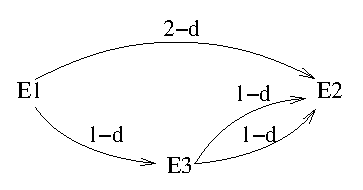
\includegraphics[width=0.4\textwidth]{figs/ks22_E1_UM_diag.eps}
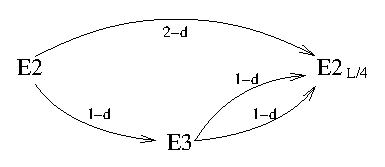
\includegraphics[width=0.4\textwidth]{figs/ks22_E2_UM_diag.eps}
\end{center}
\caption{
\PCedit{
Include here that cage of heteroclinic connections that's currently
xfig somewhere out of the repository.
    }
        }
\end{figure}


It is very unlikely that a single 1-$d$ Poincar\'e section,
can do the job, previous work\rf{Lan:Thesis,LanCvi06}
always needed several sections.

The idea is that the local unstable plane gives 2 coordinates, the
least contracting direction (or one of a complex pair) gives the 3rd.

We need to construct the backbone of heteroclinic connections
first. They are not like 3-$d$ R\"ossler and Lorenz examples:
here one spirals out,
then spirals in - hopefully there will be intelligent Poincar\'e sections
transverse to initial \EQV{2} (or {\EQV{3)} unstable manifold, mapping onto
Poincar\'e sections of trajectories leaving again
the next \EQV{3} or \EQV{2} unstable manifold.


Check next what these 2 unstable eigenvectors for \EQV{3}~\eqv\ are - when they
are equal in magnitude you expect a `star', all directions in their plane
going straight out. Do they all fall int \EQV{2}~\eqv?

% Ruslan:  10 Jul 2006
%
% 119 KB     "long_orbit.jpg"
%  88 KB     "steady_states1.jpg"
%  84 KB     "steady_states2.jpg"
% 197 KB     "rpos1.jpg"
% ----------------------------------------

For all spatial plots color axis $u \in [-3, 3]$ is the same,
same time units and spatial width $L$.
For the steady states the magnitude of the \EQV{2} is quite
a bit smaller than that of the \EQV{3}.

On the
    $[a_?,a_?]$ plane
    the $\sigma x = -x$ symmetry of \KSe\ is explicit.


steady\_states1.jpg shows the numerical evolution and, since the
traveling wave is very unstable, it disappears after awhile.
The numerically exact solution is plotted in steady\_states2.jpg

rpos1.jpg is attached as a sample.

As it looks, will not help us with partitioning, it seems, unless there is
a trajectory that hits the contracting direction - maybe
( -0.11941393,0)
head on.

Might want to look at this blowup in
the \EQV{2} slowest contraction
$   ( -0.08402656 \pm i 0.16019413)$
complex eigenvectors plane, check whether the
spiralling rotation agrees with the real/imaginary parts of eigenvalues.

Question is still - why does all of the unstable manifold of
\EQV{2}~\eqv\ go back
into
\EQV{2}~\eqv?

%%%%%%%%%%%%%%%%%%%%%%%%%%%%%%%%%%%%%%%%%%%%%%%%%%%%%%%%%%%%%%%%
\begin{figure}[t] \label{f:neighborhood2w}
\begin{center}
(a) 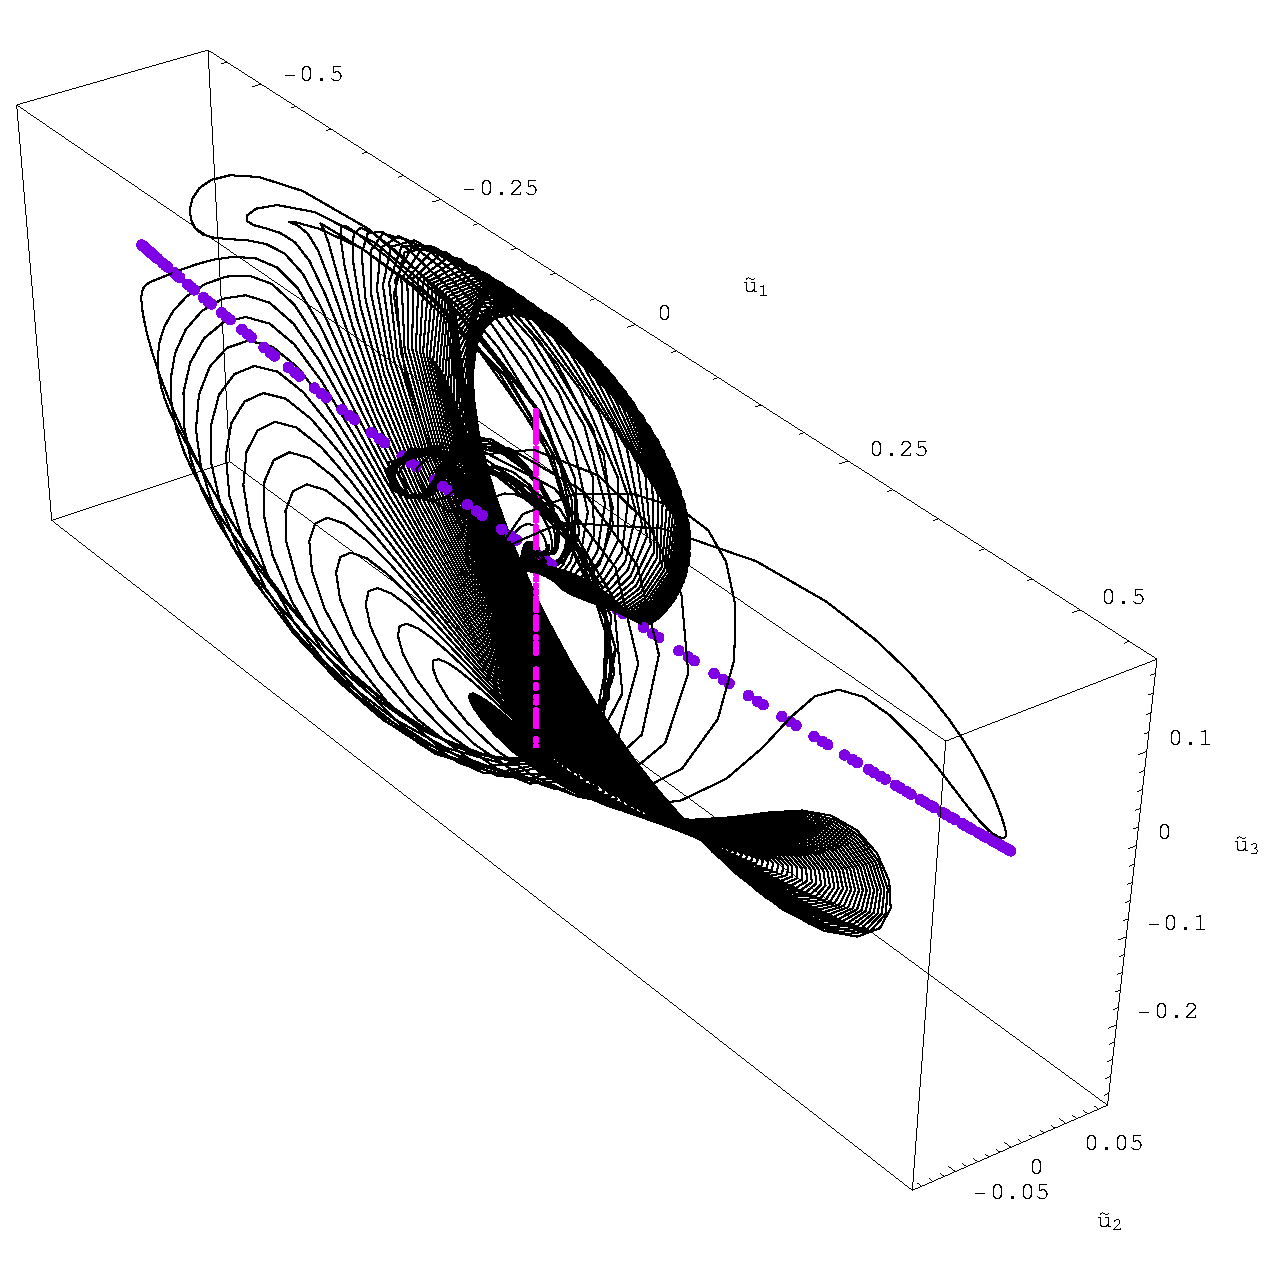
\includegraphics[width=5.0cm]{figs/L22-2w-UnsMan.eps}
\hspace{0.1in}
(b) 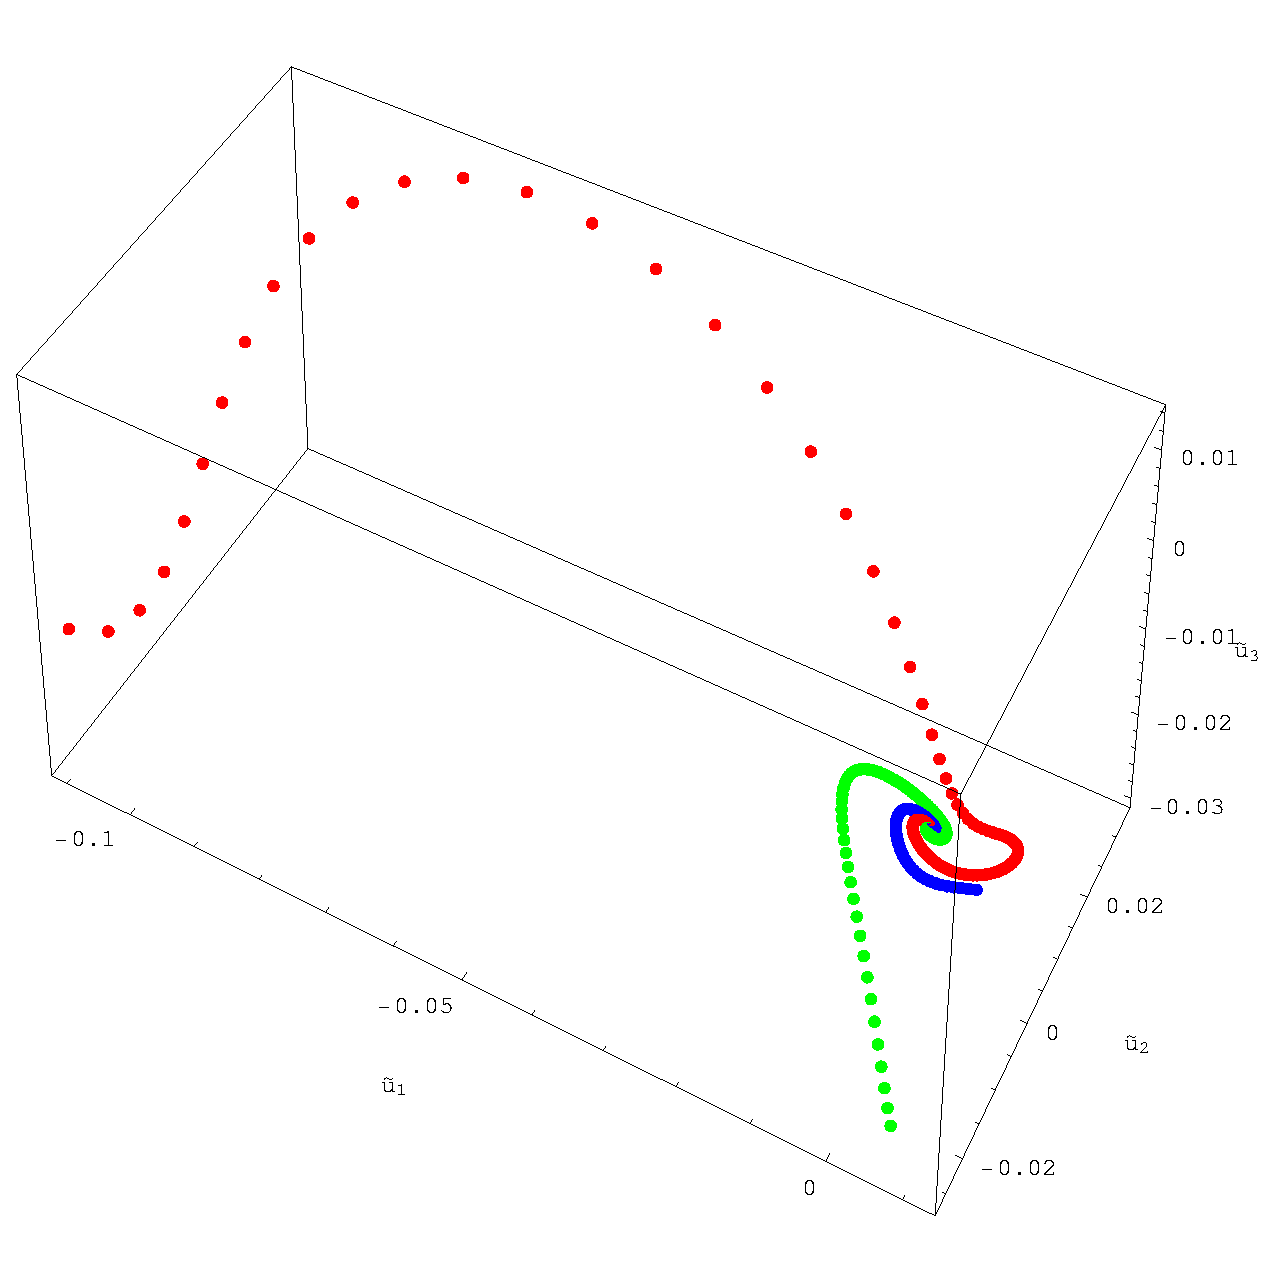
\includegraphics[width=5.0cm]{figs/L22-2w-UnsMan-BlowUp.eps}
% (b) 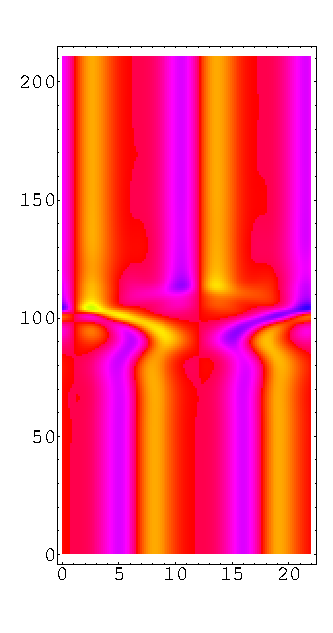
\includegraphics[width=4.0cm]{figs/L22-2w-R.eps}
\\
(c) 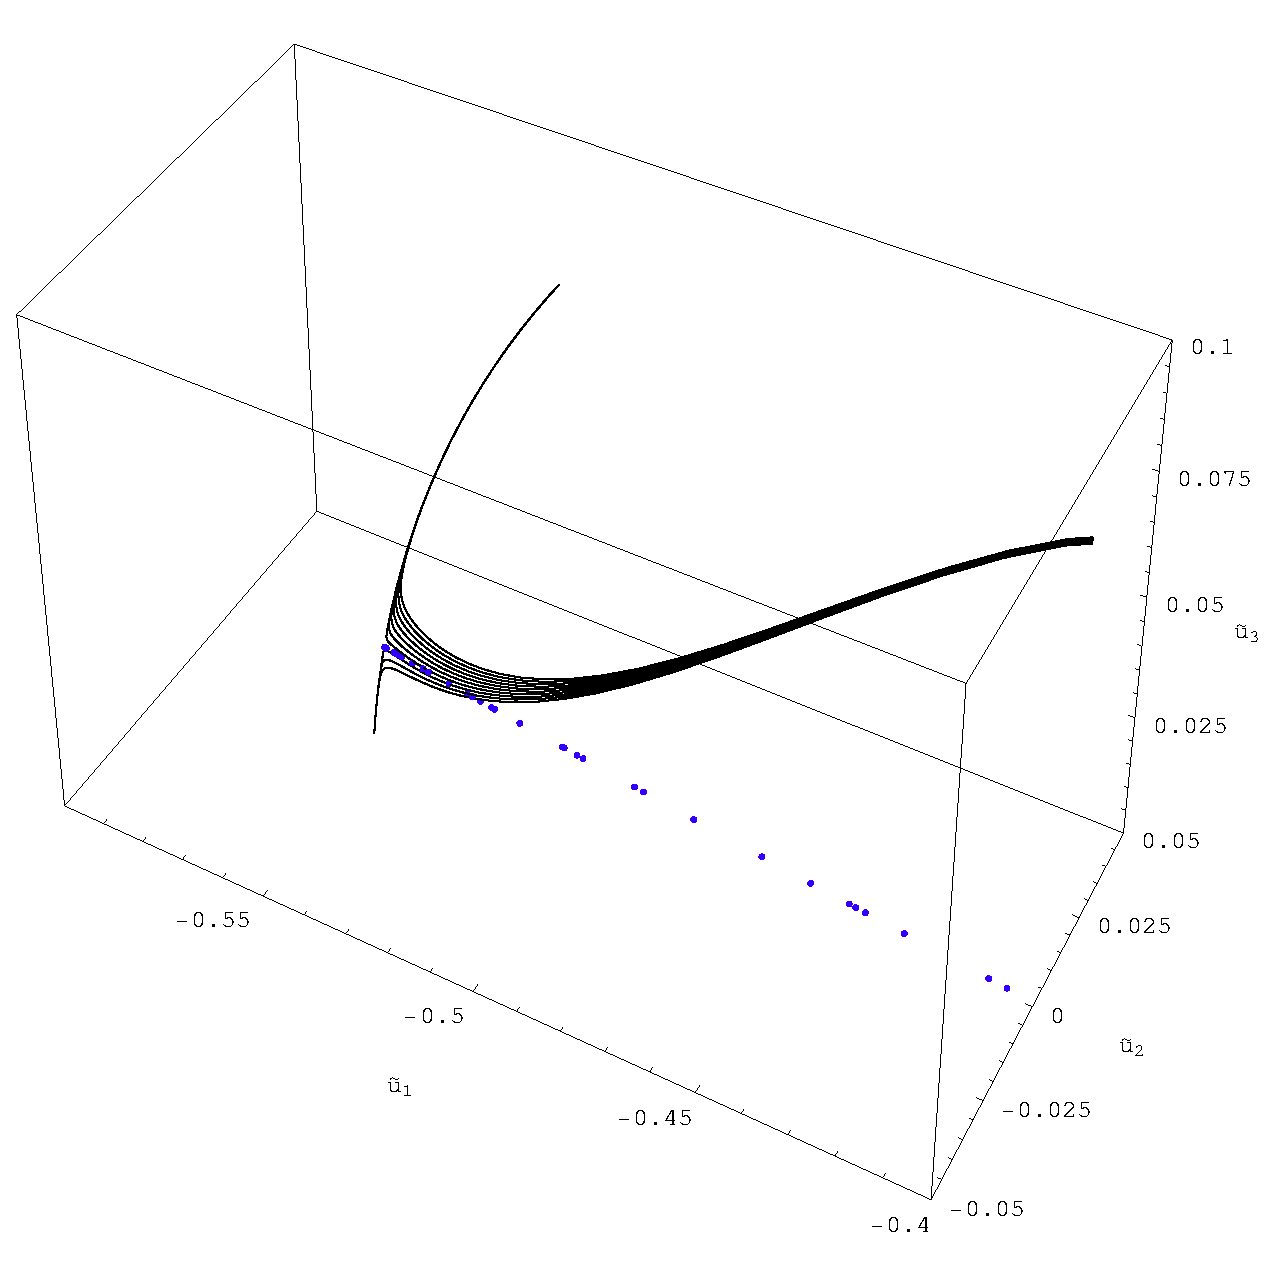
\includegraphics[width=5.0cm]{figs/L22-2w-3w-UnsMan.eps}
% (c) 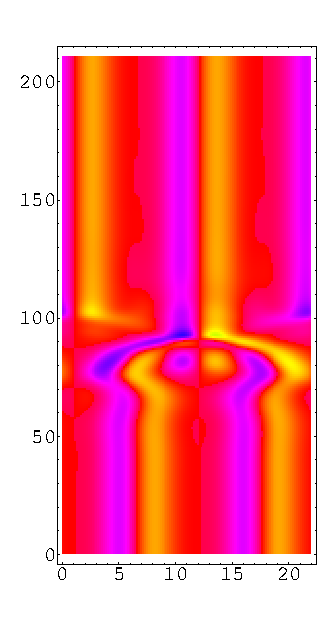
\includegraphics[width=4.0cm]{figs/L22-2w-G.eps}
\hspace{0.1in}
(d)  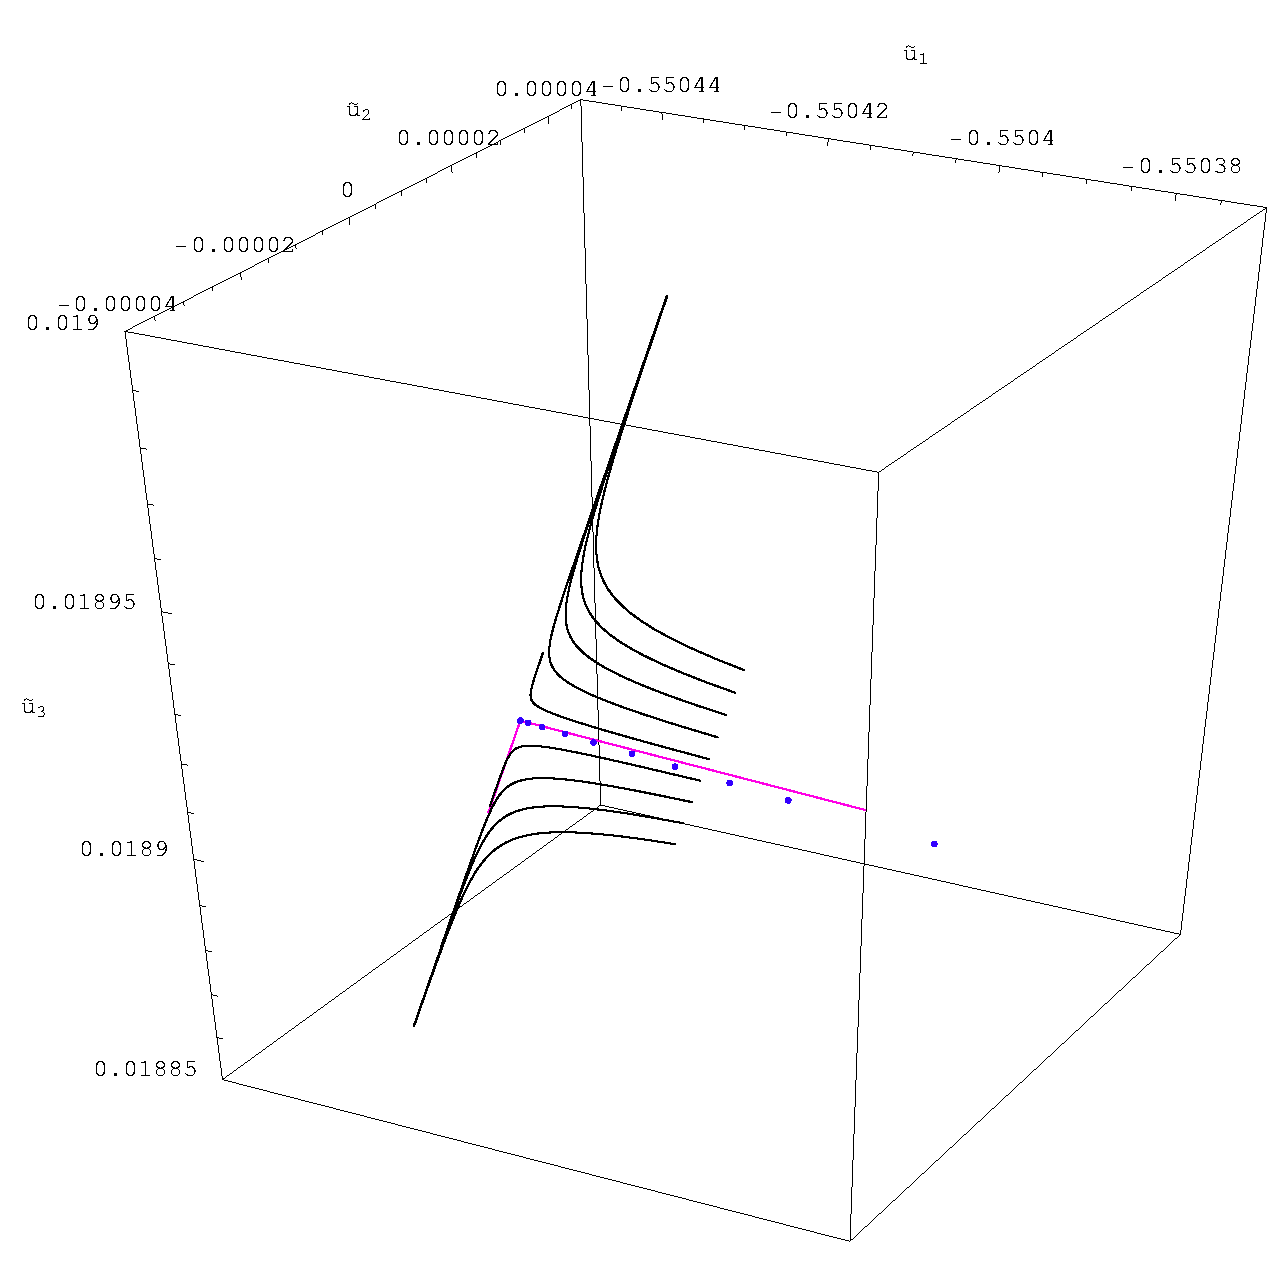
\includegraphics[width=5.0cm]{figs/L22-2w-3w-detail.eps}
% (d) 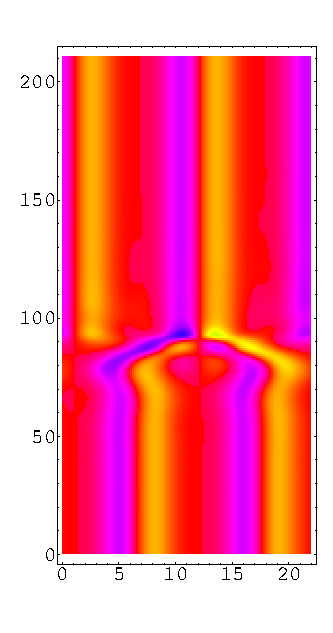
\includegraphics[width=4.0cm]{figs/L22-2w-B.eps}
\end{center}
\caption{
 Trajectories with initial conditions on the unstable subspace of
 the \EQV{2}~\eqv.
 (a) The coordinates $\tilde{u}_1$ and $\tilde{u}_2$
 are along the directions defining the unstable subspace
 and $\tilde{u}_3$  is along the real part of the eigenvector
 corresponding to the eigenvalue $-0.271122+ i\, 0.356307$.
The purple points represent the continuous family
 of
\EQV{2}~\eqva.
% Green curve belongs to \reffig{f:rpo55}(b) % rpo22-55-4-cm.eps
% rather than to  \reffig{f:rpo55}(a), % rpoEq22-55-4.eps?
(b) blowup of ``homoclinic'' descent of the unstable manifold
back into \EQV{2}~\eqv, shifted by
$L/4$.
(c) blowup of ``heteroclinic'' connection from
\EQV{2} \eqv\ to \EQV{3} \eqv, with shift
$L(1/3-1/4) = L/12$
\PCedit{(? check)}
to the neighborhood of the point near which the
unstable manifold of the
\EQV{2} \eqv\ splits. The blue points
represent the
\EQV{3} {\eqv} family.
The descent is along the eigenvector of $\Lyap_4= 0.413$,
\ESedit{(checked)}
and splitting
occurs along one of the
$\Lyap_1=\Lyap_2=0.0933$
unstable directions of the \EQV{2}~{\eqv}.
\ESedit{(checked)}
(d) same as (c), closer to the \EQV{3}~{\eqv}.
The eigendirections corresponding to $\Lyap_1$
and $\Lyap_4$ are shown in purple.
}
\end{figure}
%%%%%%%%%%%%%%%%%%%%%%%%%%%%%%%%%%%%%%%%%%%%%%%%%%%%%%%%%%%%%%%%%%

\subsection{\Reqva}

In addition to the \eqva\ , the KS system has \reqv\ solutions
(also called traveling or rotating waves in the literature).
They are characterized by a fixed function profile, $u(x)$,
moving with constant speed $c$, i.e.
\[ u(x+ct,t) = u(x, 0)\,,\quad t \in \mathbb{R}\,.\]
Because of the reflection symmetry, the \reqva\ come in pairs
related by the transformation: $u(x) \to -u(-x)$, $c \to -c$.
In Fourier space the \reqva\ are defined by the condition
\[ a_k(t)\mathrm{e}^{-iq_kct} = a_k(0)\,.\]
Differentiating this condition with respect to time, we obtain
equation for the \reqv\
\[ f_k(a) - i q_k c a_k = 0 \]
which needs to be solved for $a_k$ and $c$.

%%%%%%%%%%%%%%%%%%%%%%%%%%%%%%%%%%%%%%%%%%%%%%%%%%%%%%%%%%%%%%%%%%
\begin{figure}[t]
\begin{center}
a)\includegraphics[width=0.3\textwidth]{figs/ks22_TW1_profile.eps}
b)\includegraphics[width=0.3\textwidth]{figs/ks22_TW2_profile.eps}\\
\includegraphics[width=0.3\textwidth]{figs/ks22_TW1_orbit.eps}
\includegraphics[width=0.3\textwidth]{figs/ks22_TW2_orbit.eps}
\end{center}
\caption{
(a)
    \Reqv\ \REQV{+}{1}.
% with $L = 22$.
(b)
2nd \REQV{+}{2}, on the bifurcation branch starting
at point $M$ in \PCedit{reffig ??}.
The upper panel shows
the \reqva\ profiles. The lower panel shows evolution
of \reqva\
and its decay into generic turbulence.
Each \reqv\ has a reflection symmetric partner related by the
transformation $u(x) \to -u(-x)$.
% , $c \to -c$.
} \label{f:ks22TW}
\end{figure}
%%%%%%%%%%%%%%%%%%%%%%%%%%%%%%%%%%%%%%%%%%%%%%%%%%%%%%%%%%%%%%%%%%


\PC{split ks22\_RE1-2.eps into four, so \reffig{f:ks22TW} can be reformatted}
Consistent with the bifurcation diagram of Greene and Kim,
we find two \reqva\ with energies $E = 0.737$ and $0.350$
(labeled \REQV{\pm}{1} and \REQV{\pm}{2} from now on).
The profiles of the two \reqva\ and their time evolution
with eventual fall into the chaotic attractor are
shown in \reffig{f:ks22RE}.  The leading eigenvalues of
\REQV{\pm}{1} and \REQV{\pm}{2} are listed in \reftab{tab:RE}.
The eigenvectors
do not belong to any of the symmetric subspaces of {\KSe}
described in ???.

\begin{table}
\caption{\label{tab:RE} Eigenvalues of the \reqva.} %\ for $L=22$.}
\begin{center} \footnotesize
\begin{tabular}{ccc|ccc} \hline
  \multicolumn{3}{c}{\REQV{\pm}{1}}  & \multicolumn{3}{c}{\REQV{\pm}{2}} \\\hline
  &$\mathrm{Re} \lambda_j$ & $\mathrm{Im} \lambda_j$ & & $\mathrm{Re} \lambda_j$ & $\mathrm{Im} \lambda_j$\\\hline
  $\lambda_{1,2}$ & $0.1156$ & $0.8173$ & $\lambda_{1}  $ & $0.3370$ & \\
  $\lambda_{3,4}$ & $0.0337$ & $0.4189$ & $\lambda_{2}  $ & $0$ & \\
  $\lambda_{5}$   & $0$      &          & $\lambda_{3,4}$ &$-0.0096$ & $0.6288$\\
  $\lambda_{6}$   &$-0.2457$ &          & $\lambda_{5,6}$ &$-0.2619$ & $0.5591$\\
  $\lambda_{7,8}$ &$-0.3213$ & $0.9813$ & $\lambda_{7,8}$ &$-0.3067$ & $0.0725$\\\hline
\end{tabular}
\end{center}
\end{table}


\underline{1-\reqv\  (traveling wave).}
% Ruslan L Davidchack,  10 Jul 2006
There is a pair of \reqva\
${\nameit}1L$,
${\nameit}1R$
(traveling waves), dual under the
$u(x) \to -u(-x)$ symmetry. They are
determined numerically by
adiabatic continuation from a smaller system size
$L~\approx 12$,
where they are stable, to $L=22$
where their velocity is atypically large, $c=0.737$,

Their exponents are:
\\
$\Lyap_i \pm \theta_i =
(
\\
  0.1156222 \pm 0.817289,   \\
  0.033663 \pm 0.418909,    \\
 0.0                    ,   \\
 -0.245729                    , \\
 -0.321321 \pm 0.98126,
\cdots
)$

The pair of \reqva\
${\nameit}2L$,
${\nameit}2R$
exists for larger system sizes, but does not continue
adiabatically\rf{KNSks90} down to $L=22$.


\subsection{\Eqva, $L$ and $c$}


The $u=0$  \eqv~\EQV{0} is a point at the origin
in \reffig{f:eqvSpatial}.
At
each integer value of $\tildeL$ the origin spews out a Hopf cycle. That
might help us prove that we have all {\eqva} for $L=22$.

Each of these \eqva\ has a different value of the $E$ integration
constant.

Plot also the two \eqva\ of \eqva\ points, their
real eigenvectors and their complex eigenplanes. All {\eqva} presumably
wind around these, and as box size $L$ changes, they form continuous
families with smoothly changing $c$. One can check that by
changing $L$ a bit and using the previous \eqv\ to find the next
one.

What does the complex eigenplane continuation does for these
{\eqva} - does it produce nice heteroclinic connections, or is it
wierder? We know there is an analytic formula for a heteroclinic
connection (see \refref{Lan:Thesis}). % Lan's thesis).

The real motivation for all this is that if we understand \eqva\ as
$L \to \infty$ we might have an entry into $L = \infty$ periodic orbit
theory of KS.
\refTab{tab:L22cminus} lists the stability eigenvalues
$\eigExp[1]^-,\eigRe[2]^-\pm\eigIm[2]^-$
of \eqv\ point $c_{-}=(-\sqrt{c},0,0)$
of \refeq{eq:3dks} for $c$ corresponding to each on of \EQV{1}, \EQV{2}
 and \EQV{3} \eqva.
The period of spiraling $T_{-}=2\pi/\theta^-_2$, expansion
rate in the complex plane of spiraling
$\ExpaEig_r\approx\exp(\eigRe[2]^- T_-)$ and contraction
rate along the stable eigendirection
$\ExpaEig_1\approx\exp(\eigRe[1]^- T_-)$ are also listed.

\begin{table}[h!]
    \caption{Who ordered this table?}
\begin{center} \footnotesize
    \begin{tabular}{l|rrrrrr}
                & $E$   &$\eigExp[1]^-$ & $\eigRe[2]^-\pm\eigIm[2]^-$   & $T_m$ & $\ExpaEig_r$  & $\ExpaEig_1$  \\ \hline
        $\EQV{1}\ $ &\ 0.13 &\ -0.55    &\ $0.28\pm1.11i$       &\ 5.67     &\ 4.79     &\ 0.04 \\ \hline
        $\EQV{2}\ $     &\ 0.22 &\ -0.66    &\ $0.33\pm1.15i$       &\ 5.47     &\ 5.99     &\ 0.03 \\ \hline
        $\EQV{3}\ $     &\ 0.79 &\ -0.94    &\ $0.47\pm1.29i$       &\ 4.87     &\ 9.92     &\ 0.01
    \end{tabular}
\end{center}
\label{tab:L22cminus}
\end{table}
